% work in progress

\chapter{Expert Questionnaire}\label{chapter: expert}

	\section{Expert Selection}
	
	\section{Questionnaire}
	\subsection{Solutions Overview Draft}
	\subsection{Questions}

	\section{Results}
	
	
\chapter{Reference Implementation}\label{chapter: implementation}

This chapter focuses on the development of a reference implementation covering the \ac{vc} lifecycle, which is based on learnings of the last few chapters concerning theoretical background and opinions of experts. It is intended to directly address the lack of practical considerations of \ac{SSI} solutions in the research area, by leveraging four of the previously listed solutions that can be used to implement the \ac{vc} lifecycle. In the next sections, the complete implementation process will be described, starting with preliminary considerations and ending with results and lessons learned.

    \section{Considerations}\label{section: ri-considerations}
    % Considerations: What should be done? Why? What's important? What not? Which implementations have i chosen? Which language for reference implementation? Why API?
    As previously stated, the reference implementation should exemplarily implement four solutions in such a way that they map, based on their capabilities, the \ac{vc} lifecycle as much as possible. This enables a practical validation of the promises made by the solution providers and can thus provide a thorough insight into the existing or missing range of functionality. This way, possible blind spots or even insufficient features can be identified, which can be used to further improve the available solutions. This approach can additionally generate added value for developers who want to use \ac{SSI} technologies in their projects, since actual experiences, capabilities, and code of the individual solutions can be reused from a real implementation process.
    
    Since the results of the implementation are also to be incorporated directly into a new developer-oriented evaluation framework, there are some key considerations that must be defined beforehand. To meet the objectives described in this section, the following considerations were established:
    % Maybe add something along the lines of: MVP -> i don't care about error handling and edge cases
    \begin{itemize}
        \item \textit{Use-case agnostic}: In order to represent the \ac{vc} lifecycle as broadly and standardized as possible, the reference implementation should not be bound to the requirements and specifics of a use case. Focusing on a specific use-case could possibly lead to certain parts of the \ac{vc} lifecycle being underrepresented or not implemented at all. Such an open approach can also invite a closer look and implementation of specific facets of a technology that would have been unnecessary for a use case. This also means that the reference implementation must be accessible in such a way that it can be used relatively independently of the technology stack being used for a use case.
        \item \textit{Flexible architecture}: The reference implementation should leverage a software architecture that makes it as easy as possible to plug in new \ac{SSI} solutions. Peculiarities and complexities should be abstracted away to create a flexible and resilient architecture. 
        \item \textit{Community efforts} Since the \ac{SSI} community is very active, it should be checked beforehand which previous work can be reused for the implementation. This applies to both the architecture and the software libraries used. In this way, it can be ensured that the work does not disregard the requirements of the community and thus reality.
        \item \textit{Implementation experience}: Throughout the entire development process, objective experiences and findings should be documented and summarized. As already mentioned, these may be relevant for other developers, the solution providers, and also for the mentioned evaluation framework.
    \end{itemize}
    
    Taking these four points into account, the goal is to create a reference implementation that is as helpful as possible. The next section explores this, starting with the base implementation and community efforts to date, on which further work can be based on.
    
    \section{Base Implementation}\label{section: base-implementation}
    % Basis for Implementation: vc-http-api -> why? What is it for? What changes/ additions have to be made? Why can I hijack it? API Document!
    % Technical basis -> express app, typescript 
    A RESTful API was chosen as the basic implementation form, since it is technology-independent and can be used in various programming languages and environments. It is only necessary that HTTP requests can be sent, which allows a high degree of flexibility in later applications. 
    
    As a basis, this work is roughly based on the ideas of the W3C Credentials Community Group, which has created an unofficial draft API definition called “Verifiable Credentials HTTP API”. This describes the structure of an API with all its routes, request, as well as response bodies, which can be used for the \ac{vc} “lifecycle management”. The group defined API contracts according to the OpenAPI standard, which were originally intended to be used as a basis for verifying interoperability of \acp{vc} issued by different providers (see interoperability report from \cite{homeland_security_preventing_2020}). It is important to note that the reference implementation is based on the state of the API contract as of April 2020 (v.0.0.2-unstable), as some small things have changed since then. The contract is strongly based on the \ac{vc} standard and divides the API into resources for the three roles: Issuer, verifier, and optional holder. The includes resources for issuing and verifying \acp{vc} and \acp{VP}, deriving, as well as revoking \acp{vc}. At this point, it should be emphasized again that this is an API definition and not an actual implementation. \cite{world_wide_web_consortium_credentials_community_group_vc_2021, world_wide_web_consortium_credentials_community_group_verifiable_2021}
    
    With regard to the reference implementation, this preliminary work is quite helpful, even if it doesn't fully cover the whole \ac{vc} lifecycle. Therefore, some changes and additions have been made. A graphical representation of the API definition is shown in Figure X, which also allows testing of the individual routes.
    \newpage
    \begin{figure}[ht]
        \centering
        \makebox[\textwidth]{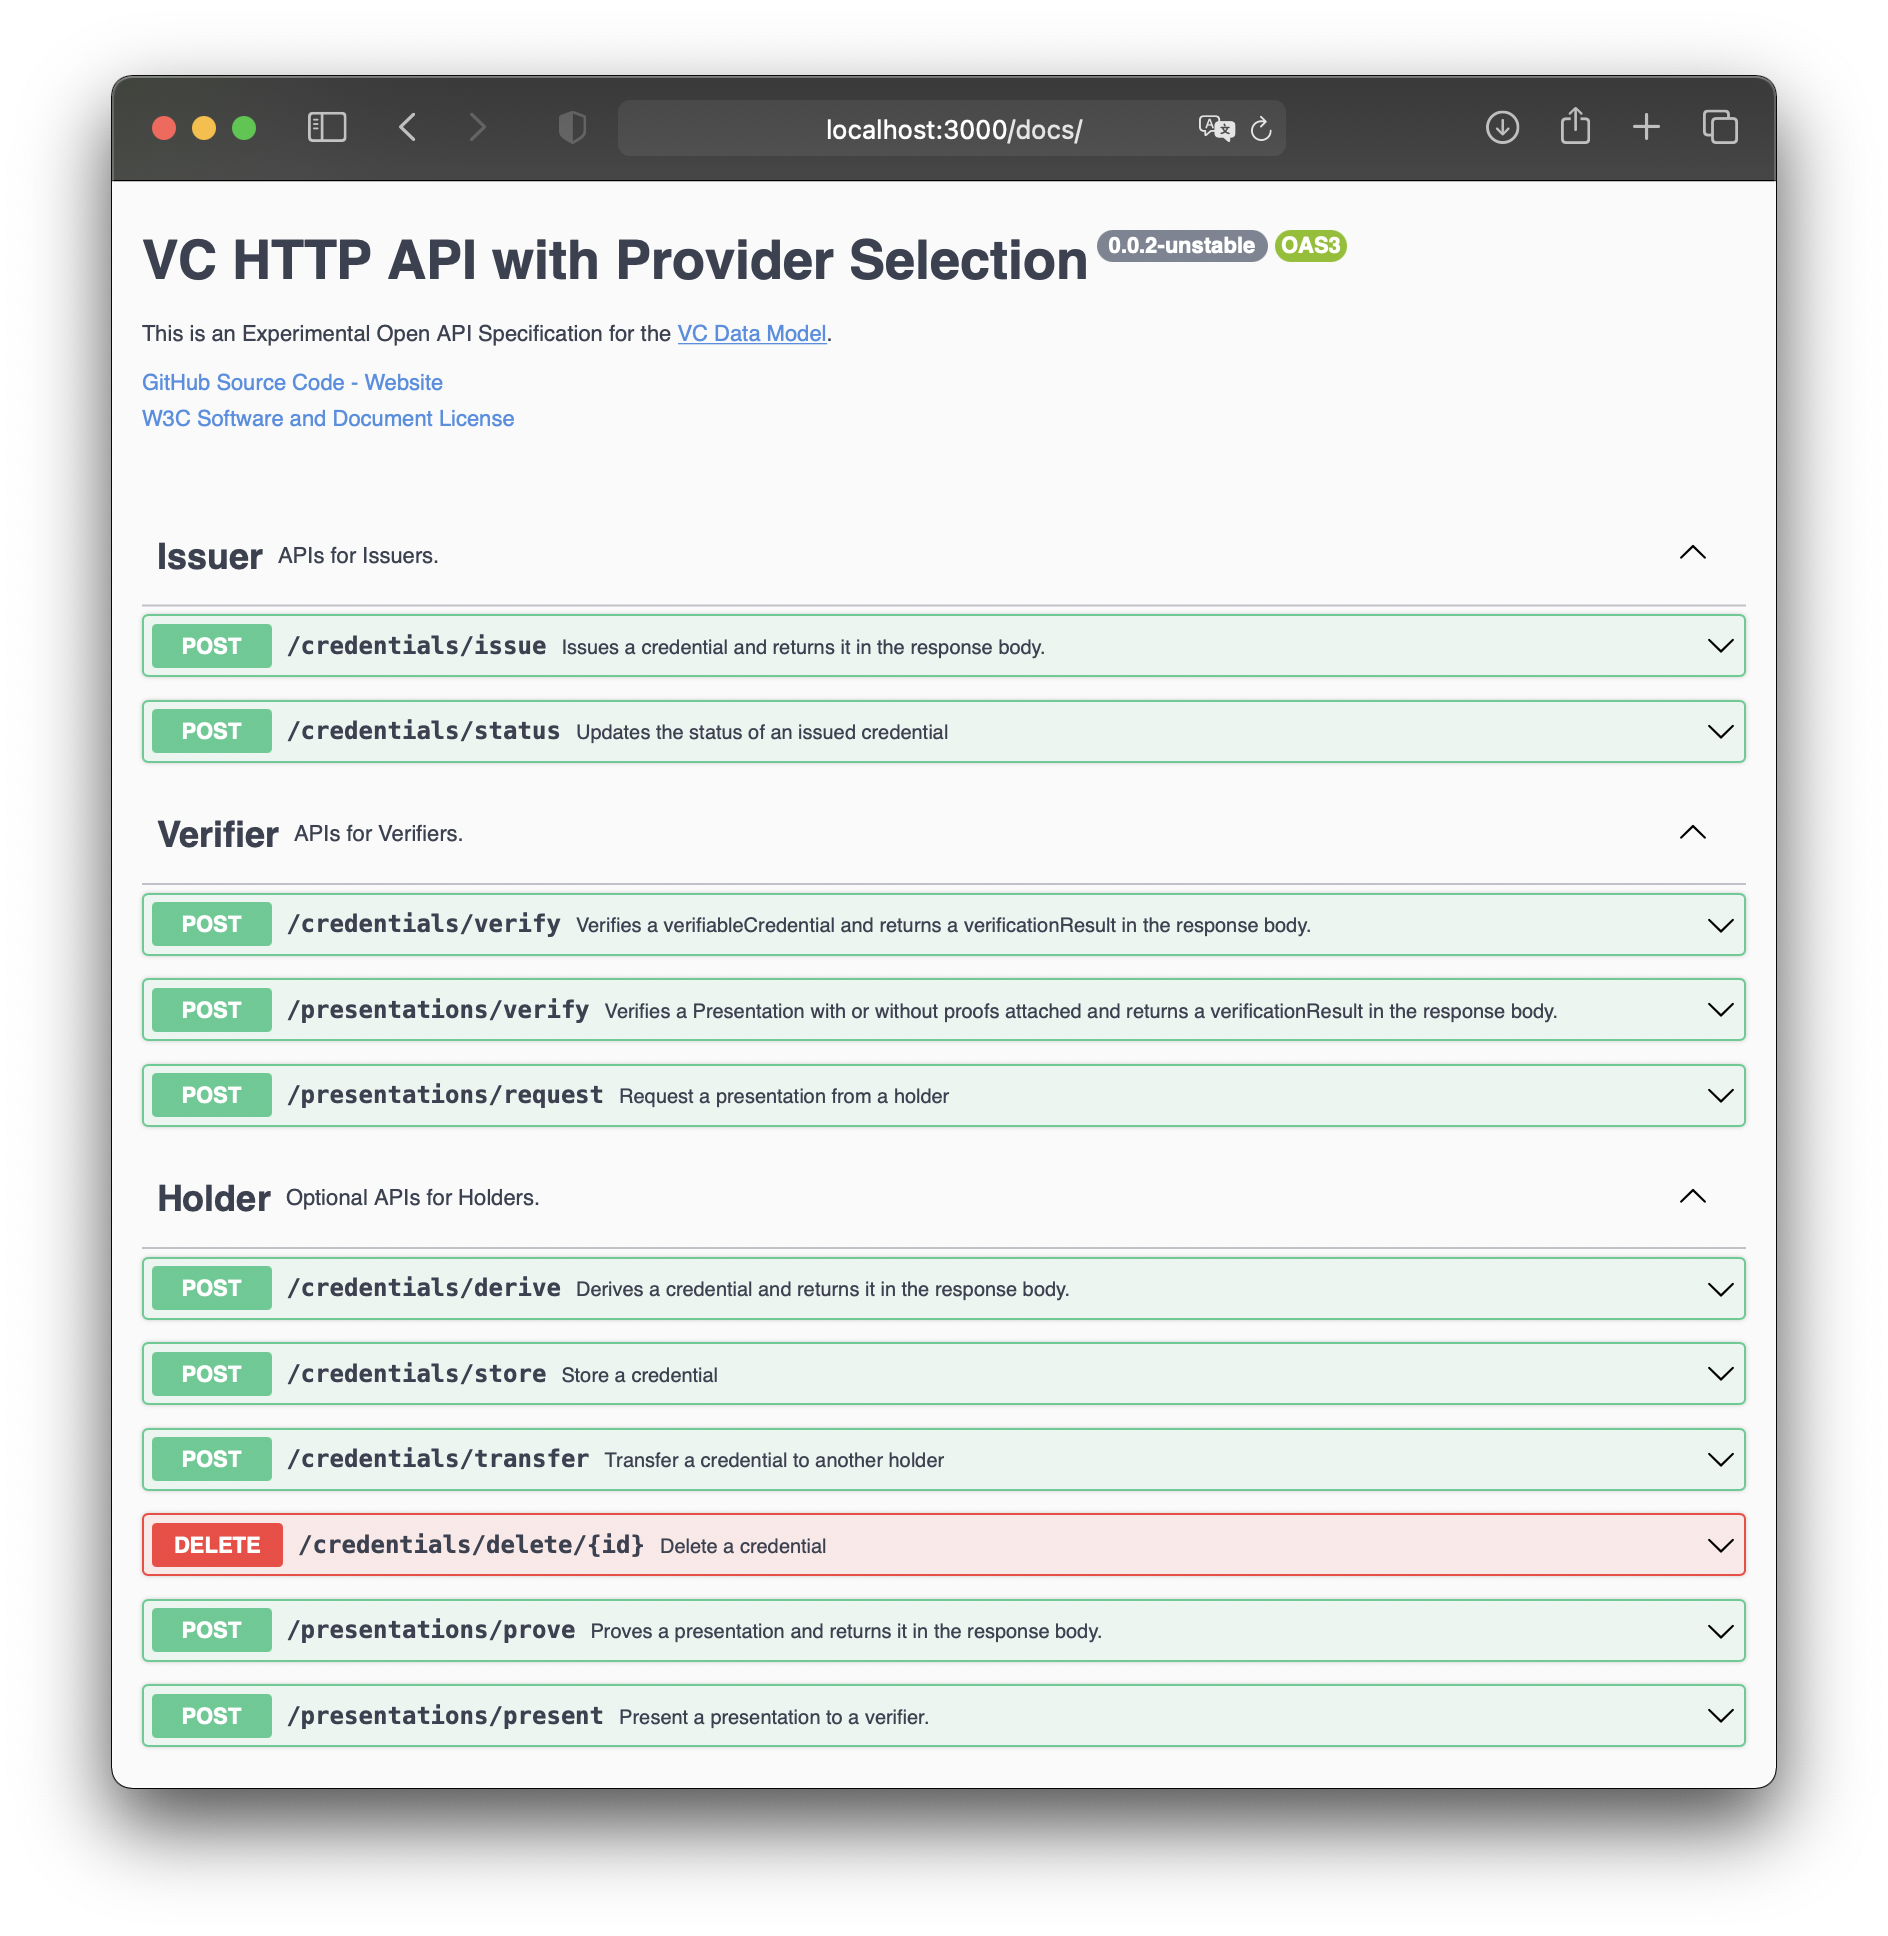
\includegraphics[width=0.9\textwidth]{thesis/img/13_api_definition.png}}
        \caption{Modified API definition (based on \cite{world_wide_web_consortium_credentials_community_group_vc_2021})}
        \label{figure: api definition}
    \end{figure}
    
    All changes made to the original definition are summarized by the following points:
    
    % TODO: might be incomplete 
    \begin{itemize}
        \item \textit{Provider selection}: Since four solutions should be addressable via the API, a query parameter was added to each route, which is based on a custom provider schema definition. Thus, it is possible to specify which solution/ provider should handle a request.
        \item \textit{Destination selection}: Another query parameter allows defining whether a request has the local or a remote agent as target. This mainly includes the issuing route for a \ac{vc}, which allows a \ac{vc} to be sent directly to the subject's agent or imported via QR code. In other cases, such as transferring \acp{vc} or presenting or requesting presentations, can be done directly via the request body. For this purpose, the schema \texttt{GenericMessage} was defined, which in its structure is very roughly based on the DIDComm data model.
        \item \textit{Added routes}: To complete the lifecycle coverage, a route to create a presentation request has been added to the Verifier and routes to save, delete, transfer of \acp{vc} and presenting \acp{VP} have been added to the Holder. For the request and response bodies, existing schemas were reused as much as possible.
        \item \textit{Response bodies}: Since some response bodies contained too much information for the requirements of the API, the schema \texttt{GenericResult} was introduced, which only contains whether the operation was successful and whether there were errors. This is the case for verifying, storing, deleting, and transferring \acp{vc} and verifying, as well as requesting/ presenting \acp{VP}.
    \end{itemize}
    
    The goal of the customizations was to ensure that the original API definition did not constrain the implementation, while retaining fundamental parts of the community work. 
    
    Based on the expert survey and observations from the IIW April 2021, the solutions Veramo from ConsenSys Software Inc, MATTR VII from MATTR Limited, Trinsic Core from Trinsic Technologies Inc, and Azure AD Verifiable Credentials from Microsoft were selected as the four solutions to be included in the reference implementation. For the implementation language, TypeScript was chosen as it was the only language where Veramo, Trinsic and Azure offer SDKs for. In addition, other basic libraries in the \ac{SSI} area are written in TypeScript or at least JavaScript and would thus integrate more easily into the implementation to possibly add missing features. Unlike JavaScript, various features of TypeScript allow cleaner and more robust code \cite[p. 87]{zammetti_modern_2020} that can simultaneously benefit from much of the existing JavaScript packages being made available from the open-source community.
    
    Building on this decision, node.js was selected as the JavaScript runtime that can be used in combination with the express.js library to develop highly scalable web applications such as APIs \cite{openjs_foundation_about_2021, openjs_foundation_express_2021}. To make TypeScript work in this environment, various dependencies such as TypeScript, ts-node, eslint, and some type definitions were installed via the Node Package Manager. The next section describes how these components and the four solutions were combined into a flexible software architecture.
    
    \section{Architecture}\label{section: architecture}
    % Software architecture, factory method pattern -> why? Describe how solutions tap into it.
    
    With regard to the considerations in section \ref{section: ri-considerations}, the factory method design pattern was chosen for the software architecture. It belongs to the creational patterns and thus influences how the instantiation process is carried out. A developer can thus decide independently of the system how, for example, objects are created, which enables a high degree of flexibility. It defines an interface or an abstract class for the creation of objects, whereby the instantiation of objects is done by subclasses instead of a class. This is useful, for example, if a class does not yet know which objects it needs to create at runtime. \cite[pp. 81, 85, 107-108]{gamma_design_1995} 
    
    This is pattern is appropriate because a request determines which solution and thus which objects have to be created. In addition, it allows the complexities of the individual solutions to be abstracted away, so that when defining the individual routes, only the concrete factory class must be called, which returns the correct object of the requested solution. This way, the routes only need to be programmed once and additional solutions can be added afterwards without having to change the code of the routes. Figure \ref{figure: factory method} shows a UML diagram that represents the concrete factory method pattern in the reference implementation. The interface \texttt{Factory} defines a method \texttt{createProvider()}, which is implemented by the class \texttt{ServiceProviderFactory}. This is the class which is instantiated, for example, in the routes and which is used to retrieve the object of a provider. A provider is the class of one of the four solutions that implements basic methods like the \ac{vc} issuance defined by the \texttt{ServiceProvider} interface.
    
    \begin{figure}[ht]
	    \centering    	    \makebox[\textwidth]{\includesvg[inkscapelatex=false, width=0.8\textwidth]{img/14_uml_ref.svg}}
        \caption{Factory method pattern in reference implementation (extracted and edited from \cite[p. 107]{gamma_design_1995})}
        \label{figure: factory method}
    \end{figure}
    
    A second pattern, which was integrated, is the Singleton design pattern. This is used in the individual concrete provider classes and allows that only one globally callable instance of a provider class can be created \cite[p. 127]{gamma_design_1995}. The rationale for this is that no more than one object is needed, caching is simplified, and multiple provider objects could lead to unforeseen complications.
    
    Looking at the complete system architecture, the previously described software architecture integrates tightly. The service provider factory sits between the routes for issuer, verifier, and holder and the concrete classes of the individual providers. Its features in the architecture can be summarized as follows and can be seen in Figure \ref{figure: sys architecture}:
    
    \begin{itemize}
        \item \textit{Veramo Provider}: The provider class requires an agent class from Veramo, which enables the integration of extensions for various functionalities. This can be, for example, the Uniresolver for resolving \acp{DID} or various services with which a connection to blockchains can be established for various actions (e.g. Infura or Microsoft's Anchoring Service). The agent also offers a REST API, which allows any actions to be executed from a remote location. Furthermore, the agent can connect to other Veramo agents on the Internet and, for example, exchange messages of any kind via DIDComm or resolve their \acp{DID}. A more detailed explanation of Veramo can be found later in subsection \ref{subsection: veramo}.
        \item \textit{MATTR Provider}: This provider communicates directly with the MATTR API, which handles any operations. Additionally, there is a callback service between the API and the provider, which can receive verification results from the MATTR platform, e.g. triggered by scanning a QR code through a mobile wallet.
        \item \textit{Trinsic Provider}: Similar to the MATTR provider, this also communicates directly with the Trinsic API and a callback service catches verification results. Thus, as with MATTR, the actual \ac{SSI} logic is outside the reference implementation.
        \item \textit{Azure Provider}: This provider is integrated into the architecture similar to MATTR and Trinsic. 
    \end{itemize}
    
    \begin{figure}[ht]
        \centering
        \makebox[\textwidth]{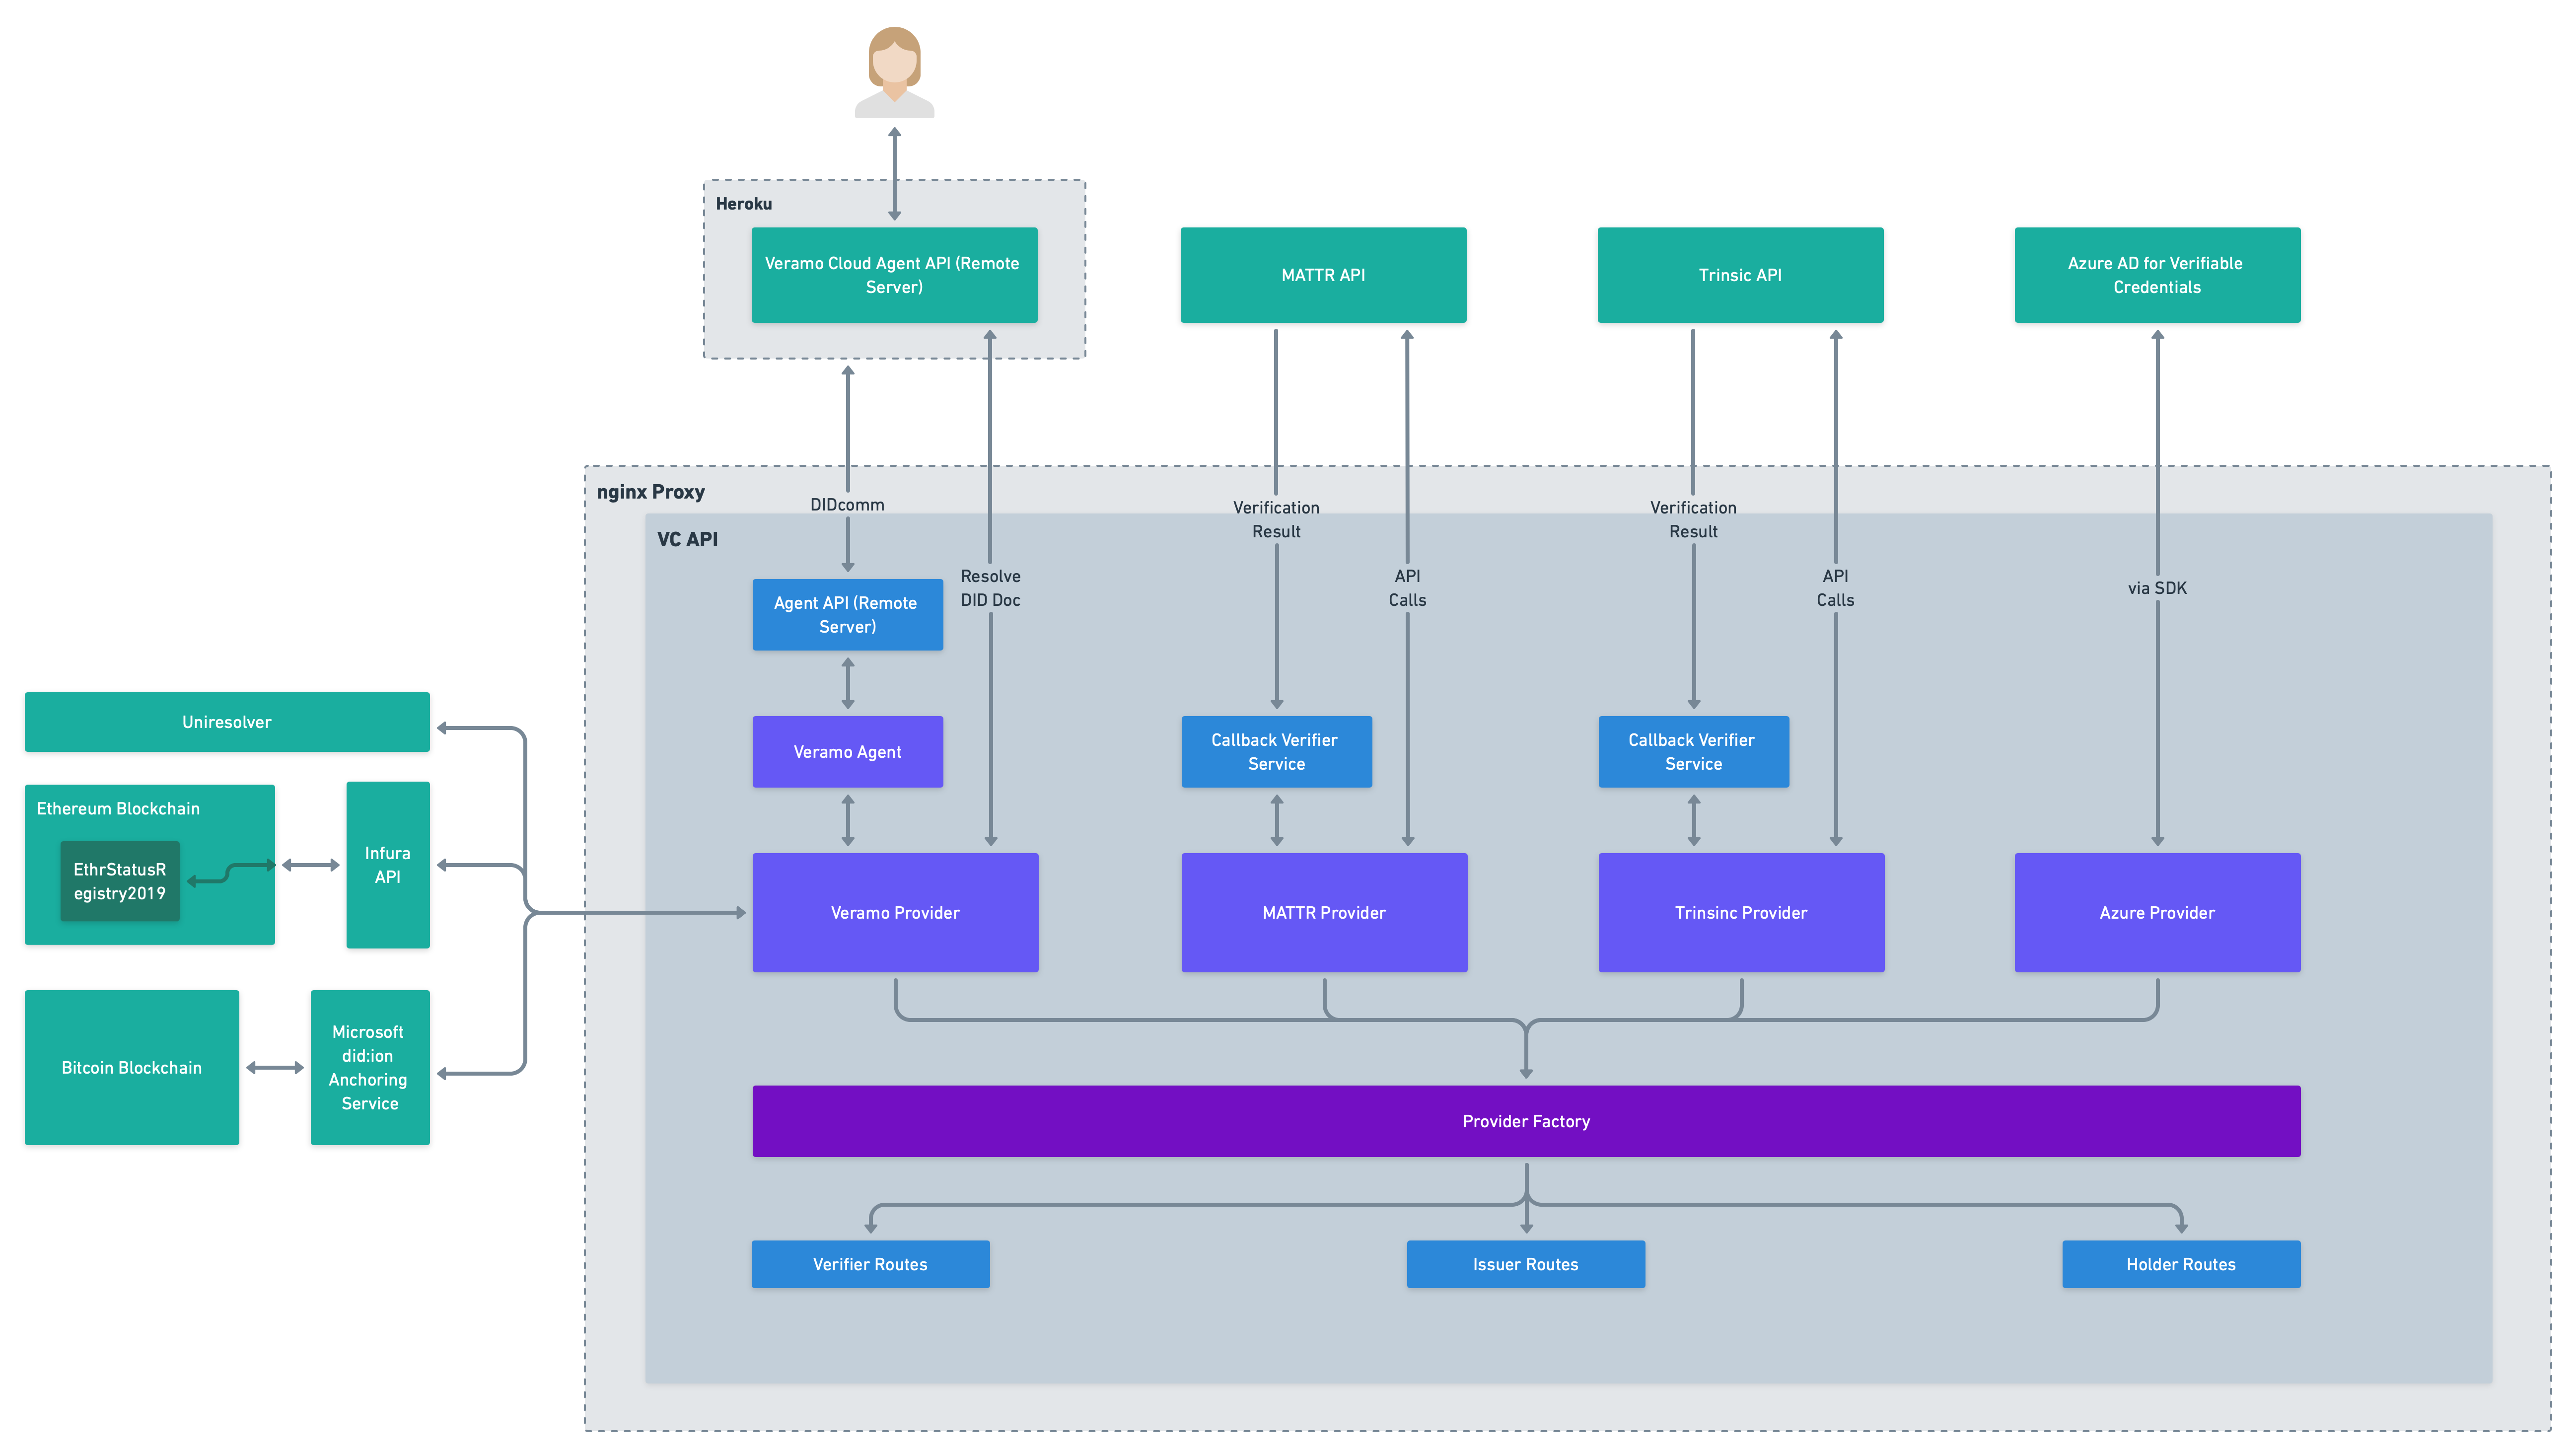
\includegraphics[width=\textwidth]{thesis/img/15_architecture.png}}
        \caption{System architecture}
        \label{figure: sys architecture}
    \end{figure}
    
    The addressed component together form the reference implementation and are enclosed only by a nginx proxy. This proxy is assigned a domain so that external components can correctly address internal components such as callback or messaging services. 
    
    \section{Solution Integration}\label{section: integration}
    % Describe implementation process, what has been done, what not. What worked, what not? What was problematic? What did I like?
    
    This section briefly introduces each of the solutions and addresses their implementation. First, however, the concepts of the last section will be discussed with regard to their implementation. The goal is to establish a conceptual skeleton into which the following subsections can be seamlessly integrated.
    
    The starting point is \texttt{index.js}, which starts the web server and thus the API via Express by bundling all routes from other files here. These are divided into the files \texttt{HolderRoutes.ts}, \texttt{VerifierRoutes.ts}, and \texttt{IssuerRoutes.ts} and implement the associated methods. Listing \ref{listing: verifier routes} shows an example of a section of \texttt{VerifierRoutes.ts}.
    \newline

\begin{lstlisting}[style=ES6, caption=Extract of verifier routes, label={listing: verifier routes}]
const router = express.Router();
const factory = new ServiceProviderFactory();

router
  .post("/credentials/verify", providerCheck, async(req, res) => {
    const query = req.query.provider.toUpperCase();
    const body = req.body.verifiableCredential;
    
    const provider = factory.createProvider(ServiceType[query]);
    const result: GenericResult =
      await provider.verifyVerifiableCredential(body);
      
    if (result instanceof Error) {
      res.status(500).send(<GenericResult>{ 
        success: false, 
        error: result.message 
      });
    } else {
      res.status(200).send(result);
    }
  })
  ...
export = router;
\end{lstlisting}

    Here, the POST method for verifying a \ac{vc} is attached to the \texttt{router} (line 10). A \texttt{providerCheck} is appended as middleware, which checks whether the provider specified in the query is indeed valid. Within the route body, the provider object is created via the \texttt{ServiceProviderFactory}, which should handle the request (line 14). This object is then used in lines 15 and 16 to verify the \ac{vc} in the request body, the result of which is then sent as a response to the requestor. By exporting the router object (line 28), all injected routes can be imported into \texttt{index.js} and made available. This example shows that no provider-specific code is present in the route code due to the factory method pattern. To demonstrate how the \texttt{ServiceProviderFactory} works, its code can be seen in listing \ref{listing: factory}.
    \newpage

\begin{lstlisting}[style=ES6, caption=Extract of service provider factory, label={listing: factory}]
export class ServiceProviderFactory implements Factory {
  createProvider(type: ServiceType): ServiceProvider {
    switch (type) {
      case ServiceType.VERAMO:
        return VeramoProvider.getInstance();
      case ServiceType.MATTR:
        return MattrProvider.getInstance();
      case ServiceType.TRINSIC:
        return TrinsicProvider.getInstance();
      case ServiceType.AZURE:
        return AzureProvider.getInstance();
      default:
        return null;
    }
  }
}
\end{lstlisting}

    The class \texttt{ServiceProviderFactory} implements the createProvider method according to the \texttt{Factory} interface. If this method is called with the desired provider (ServiceType), as e.g. in listing \ref{listing: verifier routes} line 14, then the Singleton object corresponding to the provider is returned via a switch statement. According to the factory method pattern, all provider classes implement the \texttt{ServiceProvider} interface and its signatures as concrete methods. This can be seen exemplarily in listing \ref{listing: provider}.
    \newline
\begin{lstlisting}[style=ES6, caption=Example of provider implementation, label={listing: provider}]
export interface ServiceProvider {
  deleteVerifiableCredential(identifier: string): 
   Promise<CredentialDeleteResult>;
  ...
}

export class VeramoProvider implements ServiceProvider {
  async deleteVerifiableCredential(identifier: string): 
   Promise<CredentialDeleteResult> {
    const db = new VeramoDatabase();
    const result: CredentialDeleteResult = { isDeleted: false };
    try {
      const isDeleted = await db.deleteCredential(identifier);
      result.isDeleted = isDeleted[0];
      result.message = isDeleted[1];
      return result;
    } catch (error) {
      return error;
    }
  }
  ...
}\end{lstlisting}

    In this case, the class \texttt{VeramoProvider} implements the interface \texttt{ServiceProvider} with its signatures like \texttt{deleteVerifiableCredential()} concretely, to delete a \ac{vc} from the Veramo agent database.
    
    Having described the programmatic skeleton, the following subsection describes the first solution MATTR and its integration into the reference implementation.
    
    \subsection{MATTR}\label{subsection: mattr}
    MATTR Limited is a New Zealand-based company \cite{mattr_privacy_2021} that specializes in providing solutions for “[...] a new world of digital trust.” \cite{mattr_mattr_2021-4}. This primarily includes their MATTR VII platform, which can be used to technically implement key components of an \ac{SSI} ecosystem \cite{mattr_products_2021}. According to the company, the platform can be divided into the following components: \cite{mattr_mattr_2021-2}

    \begin{itemize}
        \item \textit{VII Core}: Since MATTR is a platform solution, Core includes a variety of web APIs that serve as the foundation. This includes APIs for \acp{DID}, \acp{vc}, \acp{VP}, and secure messaging between \acp{DID}. \cite{mattr_vii_2021}
        \item \textit{VII Extensions}: These are additional components that build on VII Core, such as a bridge for OpenID Connect systems (see user-centric identities), or white label mobile wallets and SDKs. \cite{mattr_vii_2021-1}
        \item \textit{VII Drivers}: Similar to PCs, this component allows flexible integration of basic elements. This includes support for various DID methods (did:key, did:web, did:sov), crypto suites (ed25519, bls12381g2)\cite{mattr_vii_2021-2}, and storage options. \cite{mattr_vii_2021-3}
    \end{itemize}
    
    In addition, the company offers resources for developers to learn the basics of SSI \cite{mattr_resources_2021} but also comprehensive API documentation, tutorials in written and in some cases video form \cite{mattr_mattr_2021}, mobile wallets, and sample app \cite{mattr_mattr_2021-1, mattr_vii_2021}. Within the \ac{SSI} community, they participate in the development of open standards \cite{mattr_approach_2021, looker_bbs_2021} and software libraries \cite{mattr_mattr_2021-5} and have demonstrated interoperability  in the Homeland Security Plugfest in 2021 \cite{homeland_security_interoperability_2021}.
    
    With regard to the integration into the reference implementation, the generous free tier and the  well-structured documentation proved to be very helpful. Thus, a large part of the \ac{vc} lifecycle could be integrated relatively unproblematically by simply addressing the corresponding endpoints of the MATTR VII REST API. These take care of any logic and can also be used to manage \acp{DID} and their keys as well as \acp{vc}. The support of BBS+ for ZKP credentials and revocable credentials (RevocationList2020) is directly integrated into the API as well. For interactions like issuance and presentation with the MATTR mobile wallet, an OIDC provider (see user-centric identity) like Auth0 is currently necessary. Its initial setup took some time, but was feasible due to the good documentation. To receive the verification result from a mobile wallet presentation, the sample apps were used to integrate a callback service into the reference implementation. In summary, the broad coverage of the \ac{vc} lifecycle, the large number of features, and the very developer-friendly documentation with tutorials stood out positively.
    
    Nevertheless, some things were noticed that could be problematic and restrictive under certain circumstances. For example, some features are not or only partially usable in combination, such as the support of BBS+ only for credentials based on did:key. Support for additional DID methods based on public permissionless distributed ledgers such as did:ion would also be desirable, which, unlike did:key, can also include other metadata such as messaging endpoints. In addition, an SSI native implementation for interactions with mobile wallets is missing, which could theoretically take place via DIDComm. This complicates things, since the MATTR platform requires an OIDC issuer and templates for e.g. presentation to be created for each type of credential that is to be issued to a mobile wallet. However, MATTR is already working on a \ac{SSI} native solution [citation needed]. The use of the OIDC provider is also limiting, as the only way to map the OIDC attributes to the JSON-LD attributes is to use the schema.org vocabulary. Custom schemas are not supported. Finally, it should be noted that the private keys for all \acp{DID} are managed by MATTR and cannot be exported by users.
    
    The majority of the integration took place in \texttt{MattrProvider.ts}, which implements the \texttt{ServiceProvider} interface. Since this class implements any functionality via HTTP requests, listing \ref{listing: mattr verification} is an example of how this works. However, it should be noted that methods such as \texttt{issueVerifiableCredential()} are significantly more complex, as specific logic such as the distinction in issuance to a wallet or not must be considered accordingly.
    \newline
    
\begin{lstlisting}[style=ES6, caption=Example of mattr verification implementation, label={listing: mattr verification}]
async verifyVerifiablePresentation(body: VerifiablePresentation): 
 Promise<GenericResult> {
  const request = { presentation: body };
  const authToken: string = await this.getBearerToken();
  const result: GenericResult = {
   success: null,
  };

  try {
    const response = await fetch(`.../presentations/verify`, {
      method: "POST",
      body: JSON.stringify(request),
      headers: { 
        "Content-Type": "application/json", 
        Authorization: `Bearer ${authToken}` 
      },
    });
    const verificationResult = await response.json();
    result.success = verificationResult.verified;
    result.error = verificationResult.reason;
    return result;
  } catch (error) {
    return error;
  }
}\end{lstlisting}
    
    Furthermore, helper methods were implemented to generate authentication tokens for the requests or to cache QR codes for issuing \acp{vc} to mobile wallets. Especially, interactions with the latter required several extra implementations that enable the generation of issuance and presentation requests in the form of QR codes via an OIDC provider to MATTR. Starting with the issuance of a \ac{vc} to such a wallet, the type, and attributes of the \ac{vc} must be prepared at the OIDC provider and MATTR. The resulting provider ID can then simply be referenced in an issuance URL and, if desired, encoded in a QR code. This can be seen in listing \ref{listing: mattr oidc issuance}.
    \newline
    
\begin{lstlisting}[style=ES6, caption=OIDC issuance QR code generation, label={listing: mattr oidc issuance}]
private getOIDCIssuerQRCode(oidcIssuer: string): Buffer {
  if (this.issuerQrCache.has(oidcIssuer)) 
    return this.issuerQrCache.get(oidcIssuer).image;

  const qrcode: Buffer = qr.imageSync(
    `openid://discovery?issuer=${process.env.MATTR_URL}
    /ext/oidc/v1/issuers/${oidcIssuer}`,
    { type: "png" }
    );
  this.issuerQrCache.set(oidcIssuer, qrcode);
  return qrcode;
  }
}\end{lstlisting}
    \subsection{Trinsic}\label{subsection: trinsic}
    \subsection{Veramo}\label{subsection: veramo}
    \subsection{Azure AD}\label{subsection: azure}
    \section{Results}\label{section: ri-results}